\documentclass[11pt,a4paper]{article}

\usepackage[utf8]{inputenc}
\usepackage[T1]{fontenc}
\usepackage[margin=2.3cm]{geometry}
\usepackage{amsmath,amssymb}
\usepackage{graphicx}
\usepackage{float}
\usepackage{xcolor}
\usepackage{caption}
\usepackage{enumitem}
\usepackage{hyperref}

\graphicspath{{figures/explainer_10x10/}}
\captionsetup{font=small,labelfont=bf}

% Colours used in the figures, so the text can point at them.
\definecolor{fblue}{HTML}{2A78D6}
\definecolor{forange}{HTML}{EB6834}
\definecolor{faqua}{HTML}{1BAF7A}
\definecolor{boxbg}{HTML}{F3F2EE}
\newcommand{\blue}[1]{\textcolor{fblue}{\textbf{#1}}}
\newcommand{\orange}[1]{\textcolor{forange}{\textbf{#1}}}
\newcommand{\green}[1]{\textcolor{faqua}{\textbf{#1}}}

% A shaded "key idea" box.
\newcommand{\keyidea}[1]{%
  \par\medskip\noindent
  \colorbox{boxbg}{\parbox{\dimexpr\linewidth-2\fboxsep}{%
    \vspace{3pt}\textbf{Key idea.} #1\vspace{3pt}}}%
  \par\medskip}

\setlength{\parindent}{0pt}
\setlength{\parskip}{0.55em}

\title{Three Dots, One Question\\[4pt]
\large A picture guide to isosceles triangles on a $10\times10$ board}
\author{}
\date{}

\begin{document}
\maketitle

\begin{figure}[H]
  \centering
  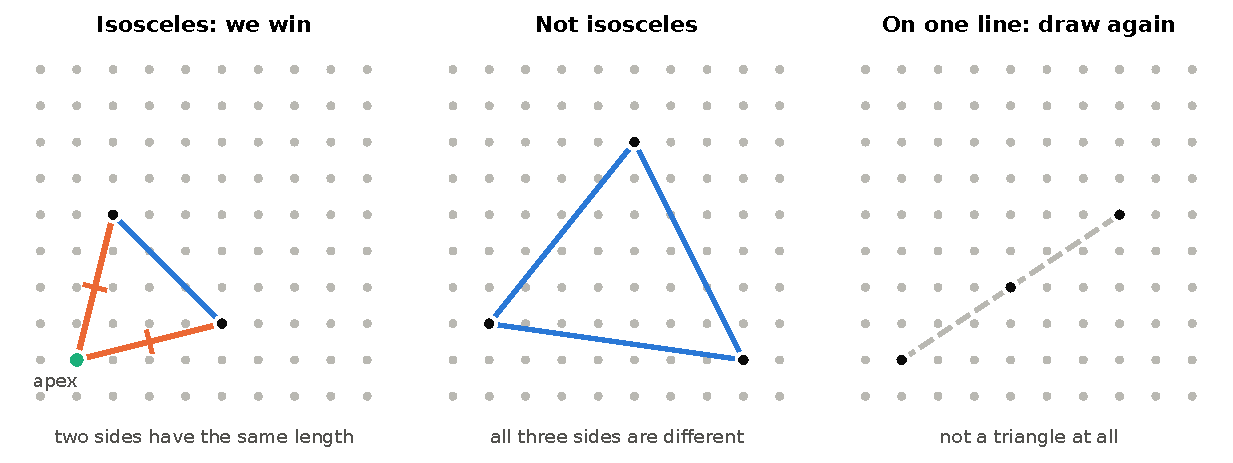
\includegraphics[width=\linewidth]{fig02_three_draws}
  \caption{The whole game in one picture. Pick three dots at random. If two
  sides are equal we win; if all sides differ we lose; if the dots fall on one
  straight line there is no triangle, and we simply pick again.}
\end{figure}

\textbf{The question.} If we keep picking three random dots, how often do we win?

\textbf{The answer.} About \textbf{7 times in every 100 rounds}, or once every
\textbf{14 rounds}. Exactly, the chance is
\[
  \frac{11\,284}{157\,252}=\frac{2821}{39\,313}\approx 0.0718 = 7.18\%.
\]

The rest of this guide shows, one picture at a time, where those two numbers come
from: $157\,252$ is the number of possible triangles and $11\,284$ the number of
isosceles ones. Each step adds only one new idea. The full proof with every detail
is in the companion note \texttt{isosceles\_10x10.tex}.

\tableofcontents

% ---------------------------------------------------------------------------
\section{The board}

\begin{figure}[H]
  \centering
  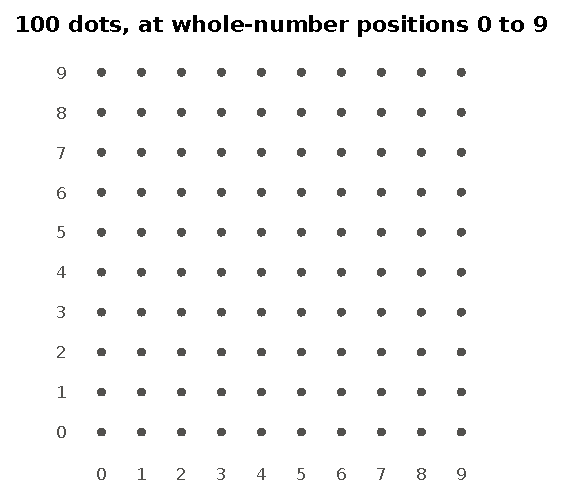
\includegraphics[width=0.45\linewidth]{fig01_board}
  \caption{The board: 10 columns and 10 rows, so $10\times10=100$ dots. Every dot
  has whole-number coordinates $(x,y)$, with $x$ and $y$ from 0 to 9.}
\end{figure}

That is all there is: a square of $100$ dots. A \emph{round} of the game picks
three different dots, each choice equally likely.

% ---------------------------------------------------------------------------
\section{What counts as a win}

A triangle is \emph{isosceles} when at least two of its sides have the same
length. In the pictures, the two equal sides are always \orange{orange} and carry
a small tick mark (the usual sign for ``these are equal''); the third side is
\blue{blue}.

\begin{figure}[H]
  \centering
  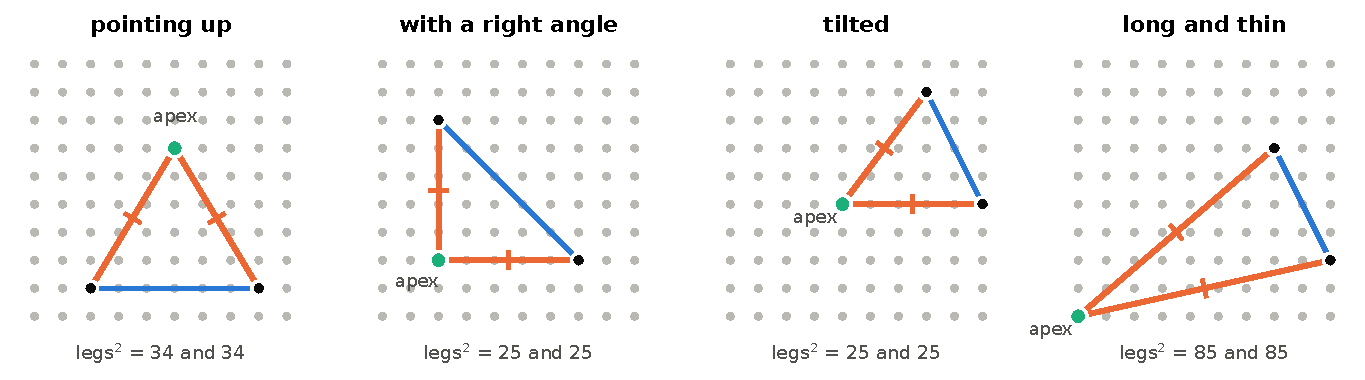
\includegraphics[width=\linewidth]{fig03_isosceles_shapes}
  \caption{Isosceles triangles come in many shapes: pointing up, with a right
  angle, tilted, long and thin. What they share is two equal sides meeting at
  one corner, the \green{apex}.}
  \label{fig:shapes}
\end{figure}

The corner where the two equal sides meet is called the \green{apex}. Keep an eye
on it: it will be the hero of the counting later.

% ---------------------------------------------------------------------------
\section{Measuring a side}

How do we know two sides are equal? We measure them with Pythagoras: walk
across, walk up, and the side is the hypotenuse.

\begin{figure}[H]
  \centering
  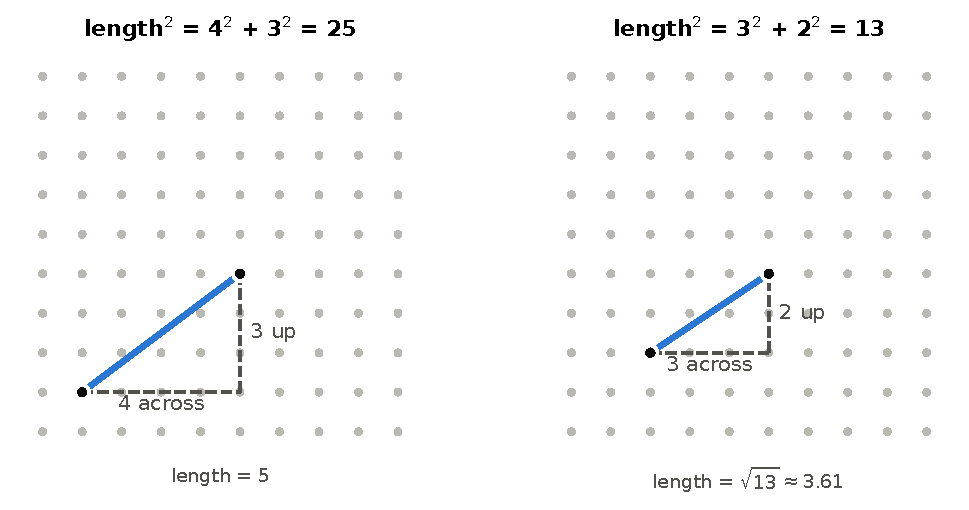
\includegraphics[width=0.8\linewidth]{fig04_pythagoras}
  \caption{Length$^2$ = (steps across)$^2$ + (steps up)$^2$. On the left the length
  is a whole number, 5. On the right it is $\sqrt{13}\approx3.61$, but its
  \emph{square} is still the whole number 13.}
\end{figure}

\keyidea{We never need the lengths themselves, only their \emph{squares}. Squared
lengths on the board are always whole numbers, so ``are these sides equal?'' is
just ``are these two whole numbers equal?''. No rounding, no doubt.}

For example, the tilted triangle in Figure~\ref{fig:shapes} has squared sides 25, 25 and 20: two
are equal, so it is isosceles.

% ---------------------------------------------------------------------------
\section{The draws that do not count}

Sometimes the three dots sit on one straight line. Then there is no triangle at
all, and the rule of the game is: throw the draw away and pick again.

\begin{figure}[H]
  \centering
  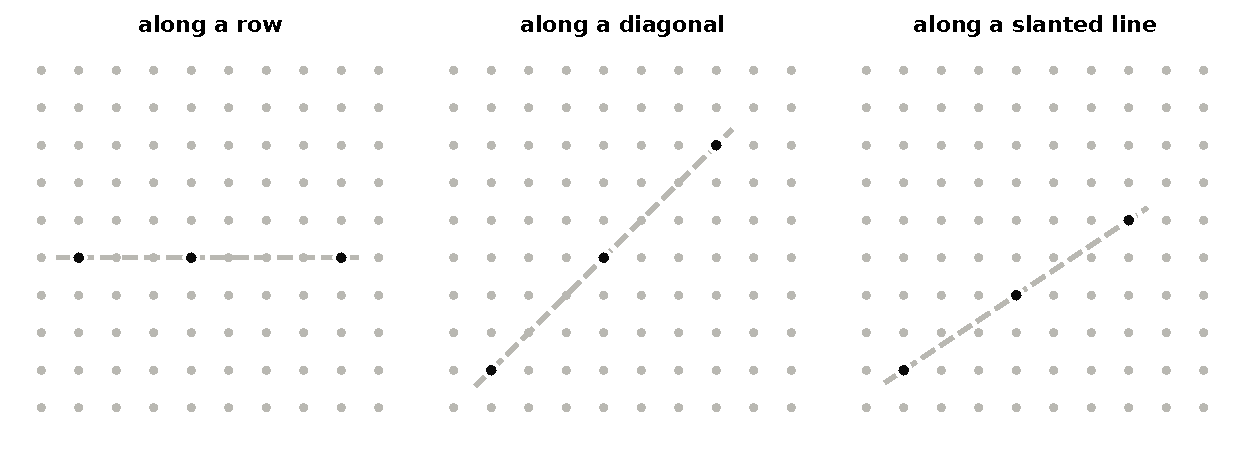
\includegraphics[width=\linewidth]{fig05_collinear}
  \caption{Three dots on one line (\emph{collinear} dots) do not make a triangle.
  The line can be a row, a diagonal, or any slanted line that passes through
  three dots.}
\end{figure}

Because collinear draws are thrown away, every \emph{real} triangle on the board
is equally likely. So the chance of winning is a simple ratio:
\[
  \text{chance of isosceles}
  = \frac{\text{number of isosceles triangles}}{\text{number of all triangles}} .
\]
The rest of the guide counts the bottom number (Sections~5--6) and then the top
number (Sections~7--13).

% ---------------------------------------------------------------------------
\section{How many ways to pick three dots?}

Pick a first dot (100 choices), a second (99 left), a third (98 left):
$100\times99\times98$ ways. But picking $A$, then $B$, then $C$ gives the same
three dots as picking $C$, $A$, $B$; each set of three dots was counted once for
each of its $6$ orders. So
\[
  \text{ways to pick 3 dots}=\frac{100\times99\times98}{6}=161\,700 .
\]
Most of these are real triangles. To find how many, we count the straight ones and
subtract.

% ---------------------------------------------------------------------------
\section{Counting the straight triples}

\paragraph{Rows and columns.} A row has 10 dots, and any 3 of them are on a line.
There are $\frac{10\times9\times8}{6}=120$ ways to choose 3 dots from a row, and
there are 10 rows, so rows give $1200$ straight triples. Columns give another
$1200$.

\paragraph{Slanted lines.} Here is a neat trick. Every straight triple has two
\emph{end} dots and one dot \emph{between} them. So pick the two end dots, and
count how many dots lie between them.

\begin{figure}[H]
  \centering
  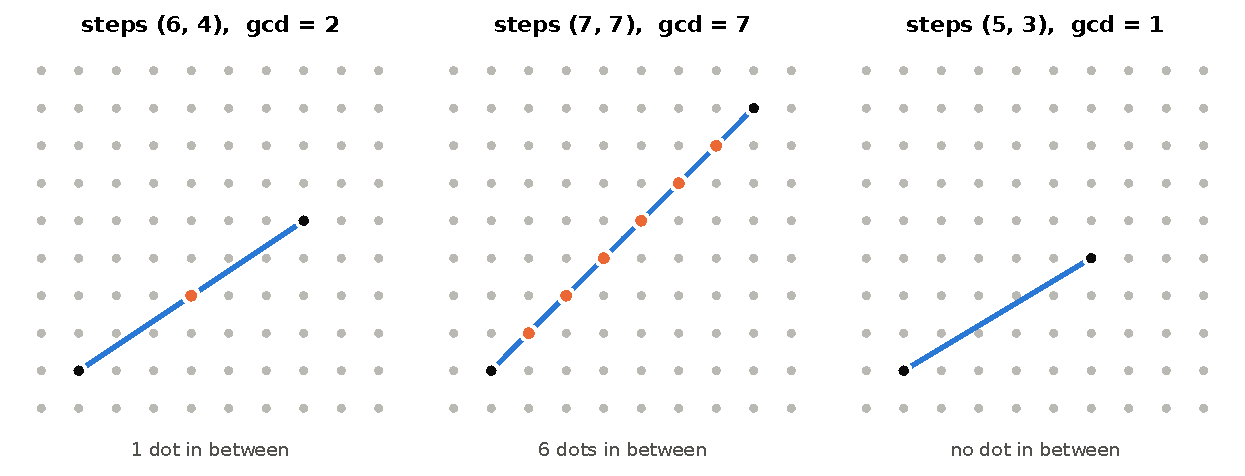
\includegraphics[width=\linewidth]{fig06_dots_between}
  \caption{To go from one dot to the other we take some steps across and some
  steps up. The number of dots strictly between them is the greatest common
  divisor (gcd) of the two step counts, minus one. Steps $(6,4)$: gcd 2, one dot
  between. Steps $(7,7)$: gcd 7, six dots between. Steps $(5,3)$: gcd 1, the line
  slips between the dots.}
\end{figure}

Each \orange{orange} dot in the middle of a segment completes one straight
triple. Adding this up over every pair of end dots on the board gives:

\begin{figure}[H]
  \centering
  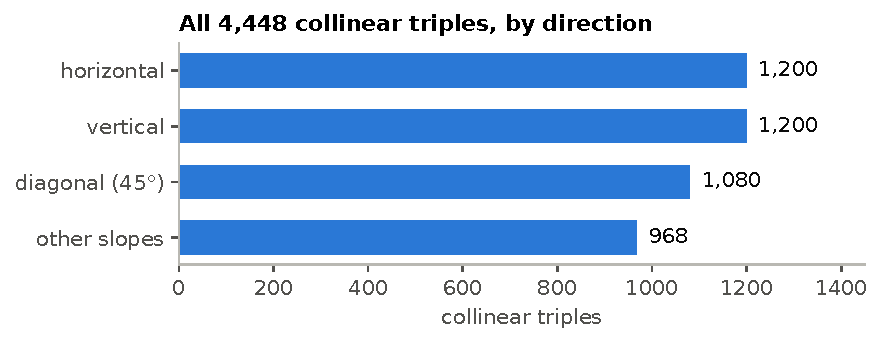
\includegraphics[width=0.75\linewidth]{fig07_collinear_count}
  \caption{All straight triples on the board, by the direction of their line.}
\end{figure}

\keyidea{There are $4448$ straight triples. So the number of real triangles is
\[
  161\,700-4448=157\,252 .
\]
That is the bottom of our fraction.}

% ---------------------------------------------------------------------------
\section{A surprising fact: no equilateral triangles}

Before counting isosceles triangles, one observation that makes the counting
clean. Could a triangle on the board have \emph{all three} sides equal?

\begin{figure}[H]
  \centering
  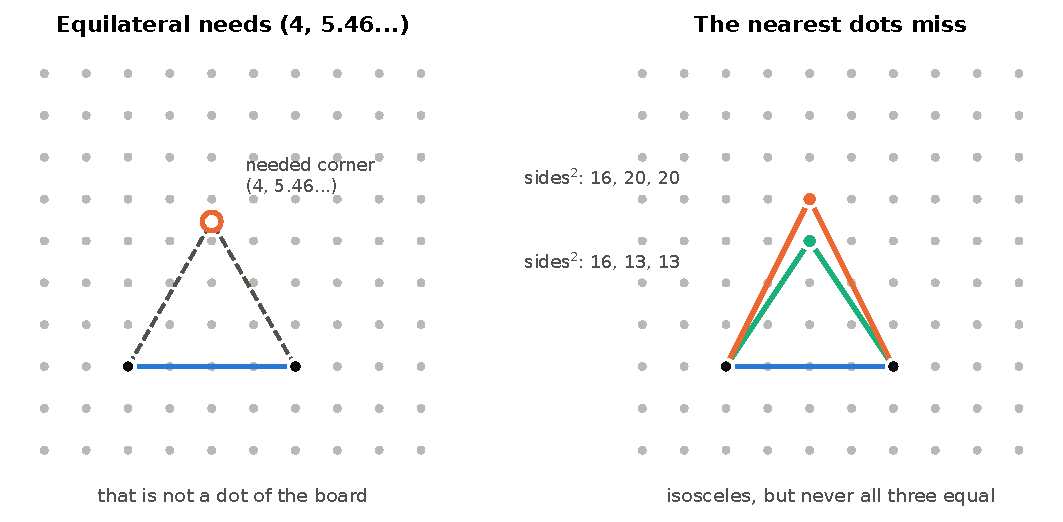
\includegraphics[width=0.85\linewidth]{fig08_no_equilateral}
  \caption{Left: an equilateral triangle on a base of length 4 needs its top
  corner at height $2\sqrt3\approx3.46$ above the base, which is between rows.
  Right: the nearest dots give isosceles triangles, never equilateral ones.}
\end{figure}

This is not bad luck with this particular base: it never works, for any base. The
area of a triangle whose corners are dots is always a whole number or a half
(you can see this by drawing a box around it and cutting off right triangles).
But an equilateral triangle with squared side $s^2$ has area
$\frac{\sqrt3}{4}s^2$, and with $s^2$ a whole number, that always contains the
irrational $\sqrt3$. The two can never match.

\keyidea{No triangle on the board is equilateral. So every isosceles triangle has
\textbf{exactly one} apex. If we count isosceles triangles by their apex, we count
each one exactly once.}

% ---------------------------------------------------------------------------
\section{The apex is the centre of a circle}

Here is the central picture of the whole guide. If the apex is equally far from
the other two corners, those two corners lie on one \emph{circle} around the apex.

\begin{figure}[H]
  \centering
  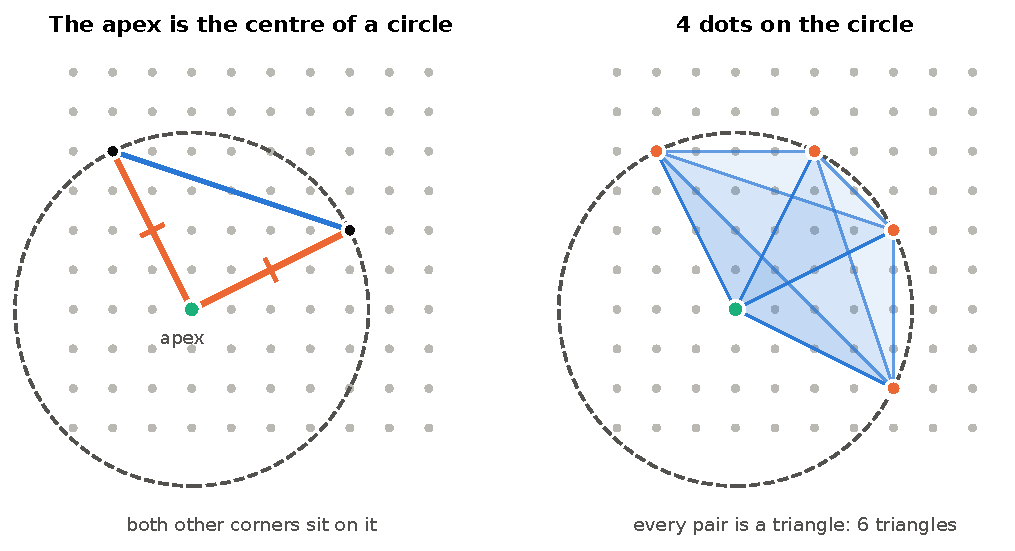
\includegraphics[width=0.85\linewidth]{fig09_apex_circle}
  \caption{Left: an isosceles triangle with apex $(3,3)$; both other corners lie
  on the dashed circle of squared radius 20. Right: this circle passes through 4
  dots, and \emph{any} two of them, together with the apex, form an isosceles
  triangle: 6 triangles in all.}
\end{figure}

\keyidea{To count the isosceles triangles with a given apex: look at each circle
around it, count the dots on that circle, and count the \emph{pairs} of those
dots. A circle with $k$ dots gives $\frac{k(k-1)}{2}$ pairs: 2 dots give 1 pair,
3 give 3, 4 give 6, 8 give 28.}

% ---------------------------------------------------------------------------
\section{Seeing the circles on the board}

Circles are easy to spot once we write, on every dot, its squared distance from
the apex. Dots showing the same number are on the same circle.

\begin{figure}[H]
  \centering
  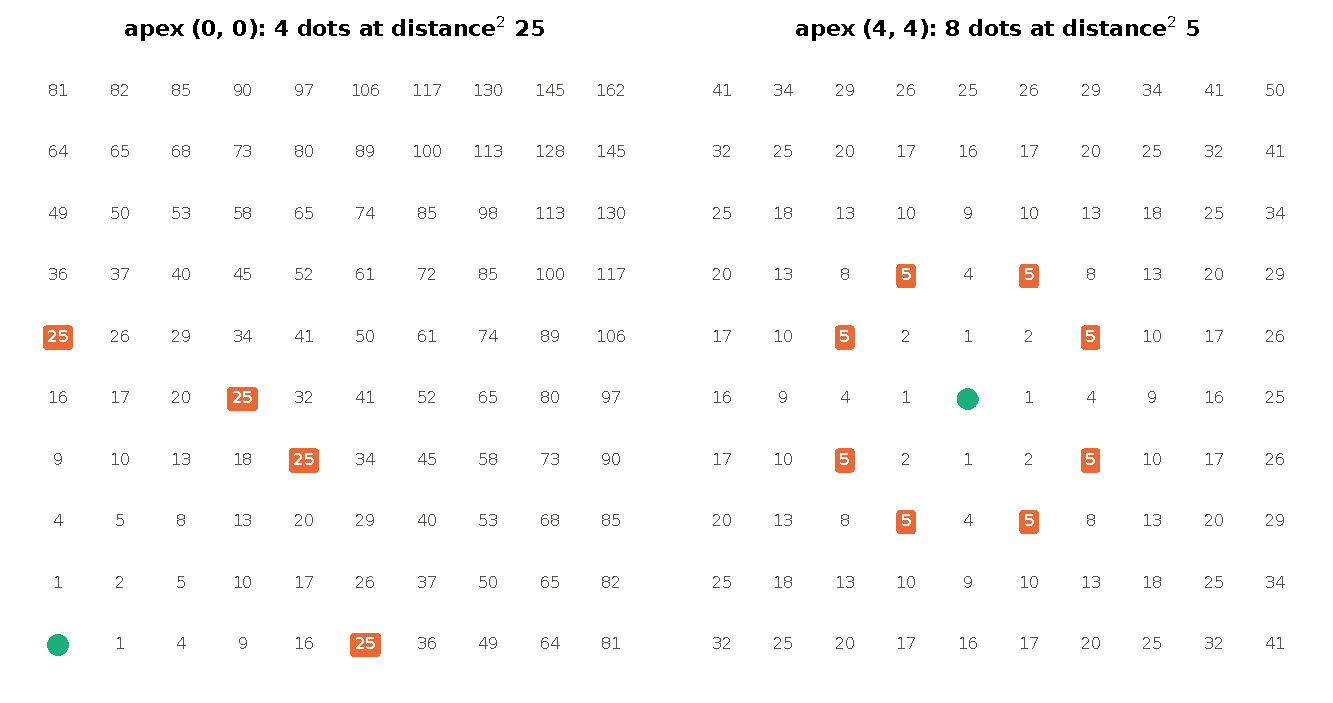
\includegraphics[width=\linewidth]{fig10_distance_numbers}
  \caption{Every dot labelled with its squared distance to the \green{apex}.
  Left, apex in the corner: the number 25 appears 4 times. Right, apex near the
  centre: the number 5 appears 8 times.}
\end{figure}

Look at the two boards side by side. In the corner, most numbers appear only once
or twice. Near the centre, numbers repeat a lot: the pattern is symmetric in every
direction, so each number shows up 4 or 8 times. More repeats means more pairs,
which means more isosceles triangles.

% ---------------------------------------------------------------------------
\section{Working out one apex: the corner}

Take the apex at the corner $(0,0)$. Its pairs come in two kinds.

\begin{figure}[H]
  \centering
  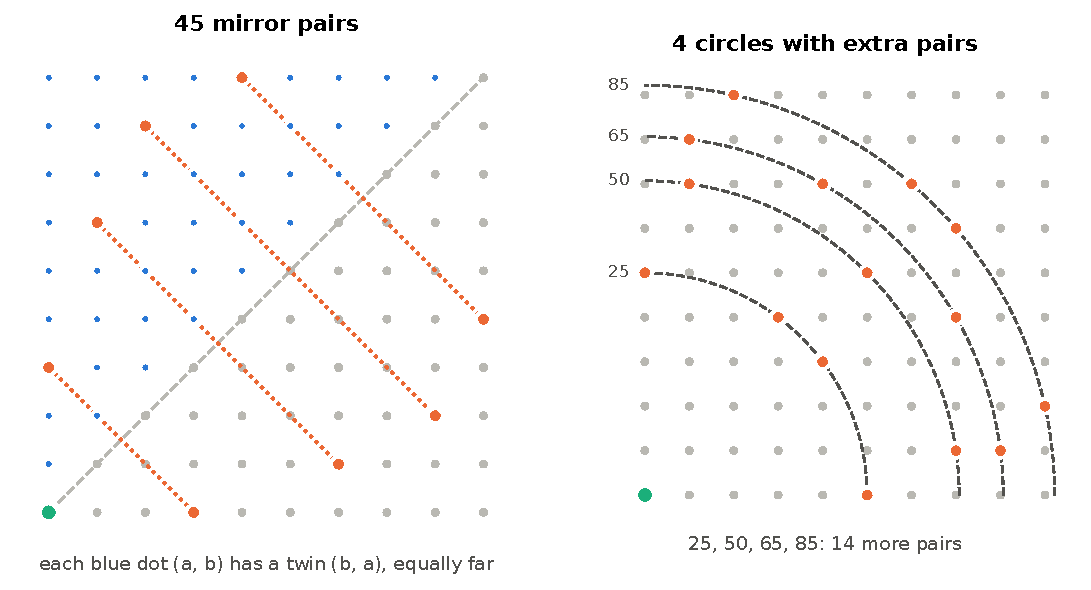
\includegraphics[width=0.85\linewidth]{fig11_corner_pairs}
  \caption{Left: the dot $(a,b)$ and its mirror image $(b,a)$ across the diagonal
  are always equally far from the corner. The \blue{blue} dots above the
  diagonal each have such a twin: 45 pairs. Right: four circles carry extra dots
  that are not mirror twins, giving 14 more pairs.}
\end{figure}

\begin{itemize}[nosep]
  \item \textbf{Mirror pairs.} There are 45 dots above the diagonal, so 45 pairs.
  \item \textbf{Lucky circles.} Some numbers can be written as a sum of two squares
    in two different ways, for example $25=0^2+5^2=3^2+4^2$. The circle of
    squared radius 25 then carries the dots $(0,5),(5,0),(3,4),(4,3)$: besides the
    2 mirror pairs, the 4 pairs that mix them are new. On the board this happens
    for $25,\ 50,\ 65$ and $85$ (for 50, the second way is $5^2+5^2$, a dot on the
    diagonal), and it adds $4+2+4+4=14$ pairs.
\end{itemize}
So the corner is the apex of $45+14=\mathbf{59}$ isosceles triangles.

% ---------------------------------------------------------------------------
\section{Corner versus centre}

A chart makes the difference between the corner and the centre obvious.

\begin{figure}[H]
  \centering
  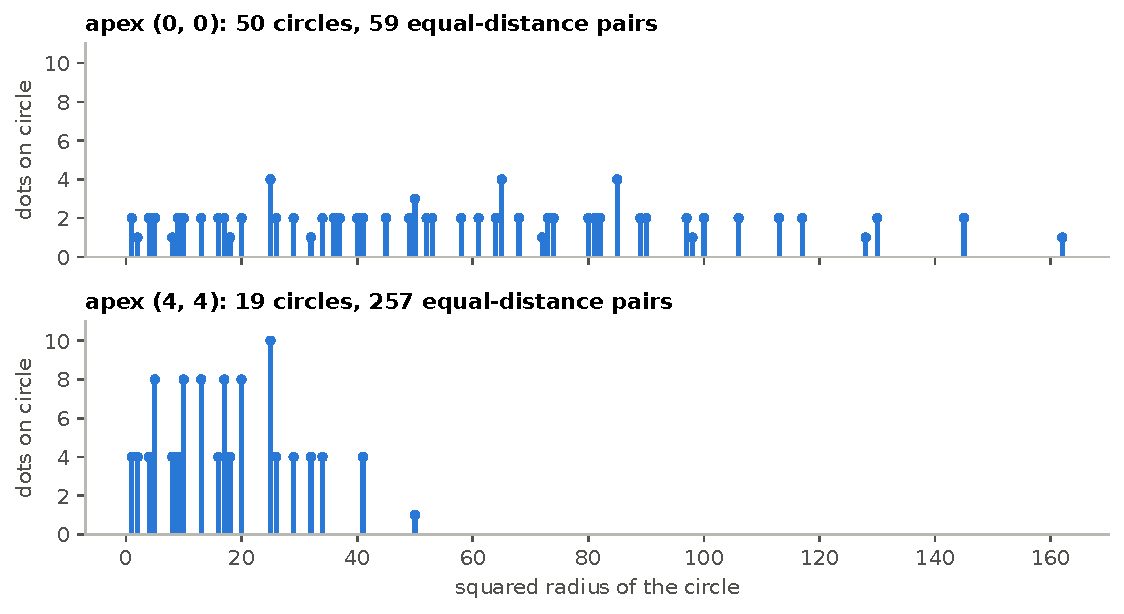
\includegraphics[width=0.9\linewidth]{fig12_ring_sizes}
  \caption{Each bar is one circle around the apex, and its height is the number
  of dots on it. The corner has many circles with only 1 or 2 dots. The centre
  has fewer circles, but they are crowded with 4, 8 or even 10 dots, so they
  produce many more pairs: 257 against 59.}
\end{figure}

Why? Around a corner dot, most of every circle falls \emph{outside} the board. Only
a quarter of each circle is left. Around a central dot, almost every circle is
complete.

% ---------------------------------------------------------------------------
\section{One last correction: equal, but straight}

There is a catch. Two dots can be equally far from the apex but on
\emph{opposite sides} of it, on one straight line. Then the apex is exactly the
midpoint, and the three dots are not a triangle.

\begin{figure}[H]
  \centering
  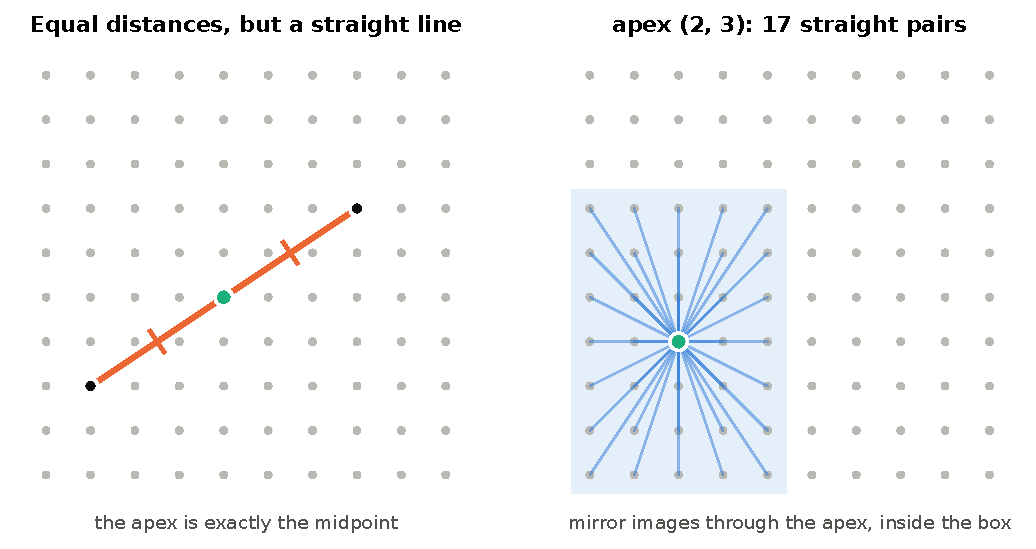
\includegraphics[width=0.85\linewidth]{fig13_midpoint}
  \caption{Left: equal distances, but the three dots are on a line. Right: for
  the apex $(2,3)$, every dot in the shaded box has a mirror image through the
  apex that is still on the board. These 17 pairs must be removed.}
\end{figure}

How many such pairs does an apex have? Draw the largest box centred at the apex
that fits on the board; every dot in it pairs with its mirror image through the
apex. A corner has none. The centre $(4,4)$ has 40. So the centre is the apex of
$257-40=\mathbf{217}$ isosceles triangles. Over all 100 apexes, 1200 straight
pairs are removed.

% ---------------------------------------------------------------------------
\section{Every dot as the apex}

Now repeat the count with every one of the 100 dots as the apex.

\begin{figure}[H]
  \centering
  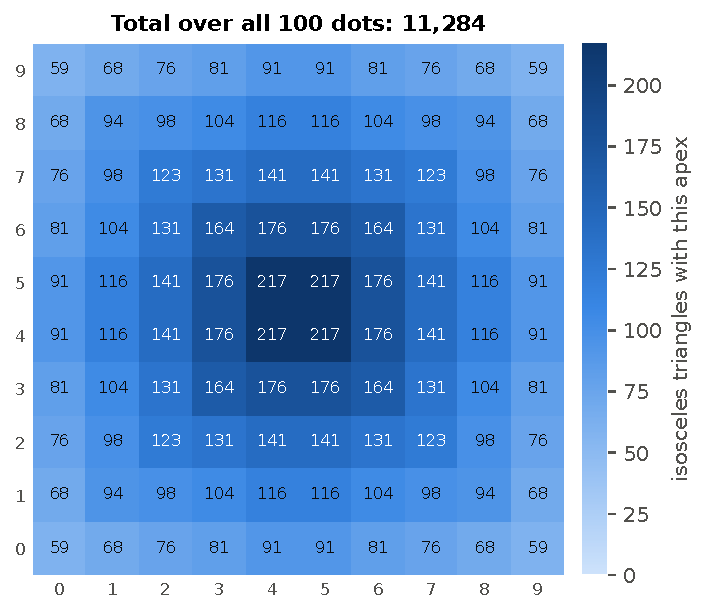
\includegraphics[width=0.62\linewidth]{fig14_apex_heatmap}
  \caption{The number of isosceles triangles with each dot as apex. Darker means
  more. The corners are the lightest (59), the four central dots the darkest
  (217). The map looks the same after turning or flipping the board, so only 15
  different numbers appear.}
\end{figure}

\keyidea{Adding the 100 numbers in the map gives
\[
  \text{isosceles triangles}=11\,284 .
\]
That is the top of our fraction.}

% ---------------------------------------------------------------------------
\section{The answer}

\begin{figure}[H]
  \centering
  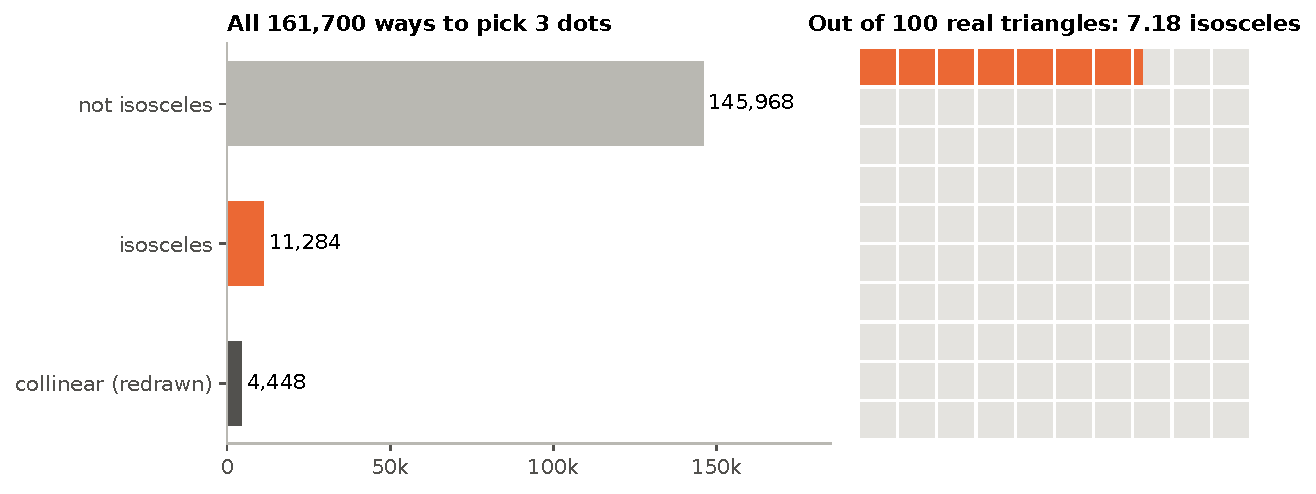
\includegraphics[width=\linewidth]{fig15_where_triples_go}
  \caption{Left: where all $161\,700$ ways of picking three dots end up. Right:
  out of every 100 real triangles, a bit more than 7 are isosceles.}
\end{figure}

Putting the two counts together:
\[
  \text{chance of isosceles}=\frac{11\,284}{157\,252}=\frac{2821}{39\,313}
  \approx0.07176 .
\]
Roughly \textbf{7 wins in every 100 rounds}, or \textbf{one win every 14 rounds}.

\begin{figure}[H]
  \centering
  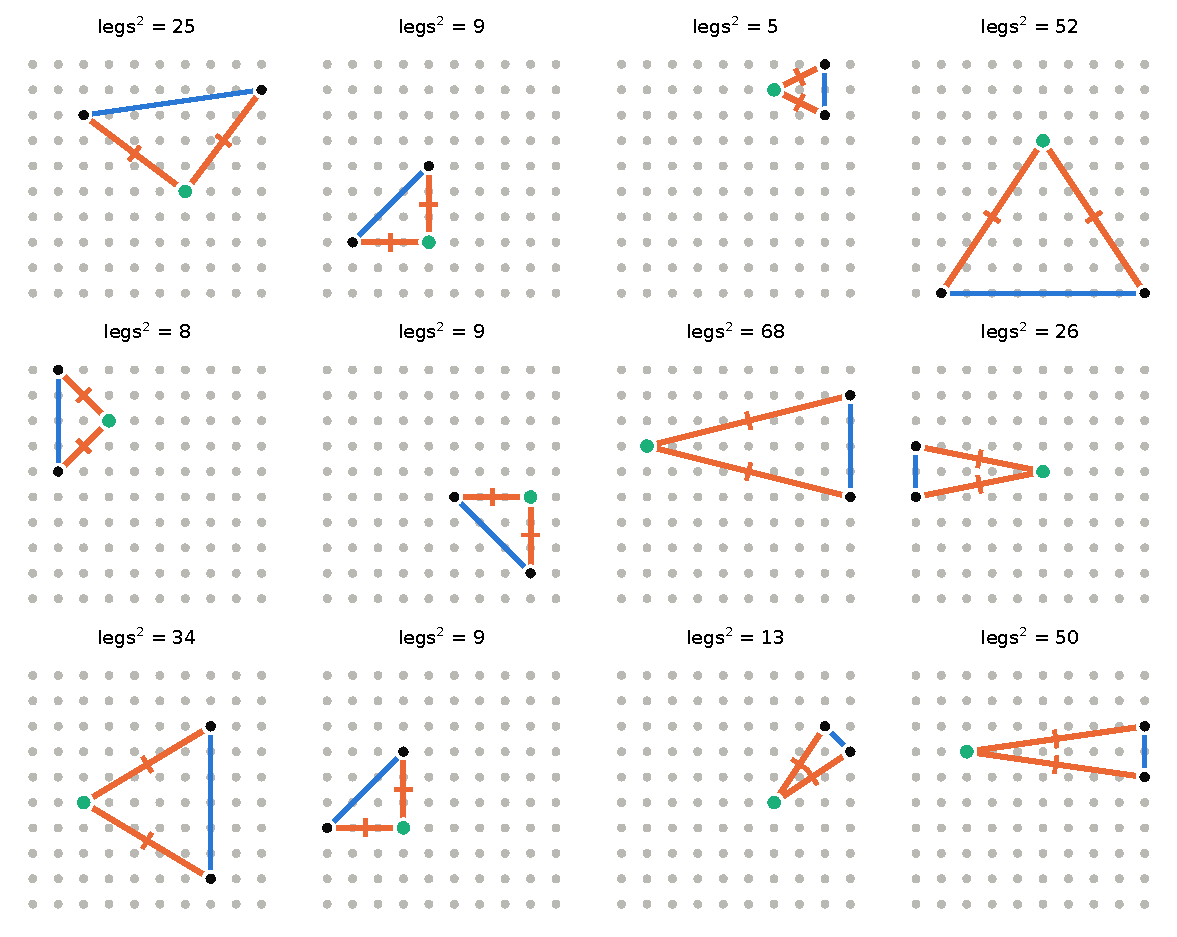
\includegraphics[width=0.9\linewidth]{fig18_random_isosceles}
  \caption{A dozen winners, found by actually drawing random dots. Notice how
  varied they are: big and small, upright and tilted, and several right-angled
  ``half squares'' (legs$^2$ = 9 and 8).}
\end{figure}

% ---------------------------------------------------------------------------
\section{Checking by playing the game}

A count this long deserves a check. So we let a computer play the game many
times and simply record how often it wins.

\begin{figure}[H]
  \centering
  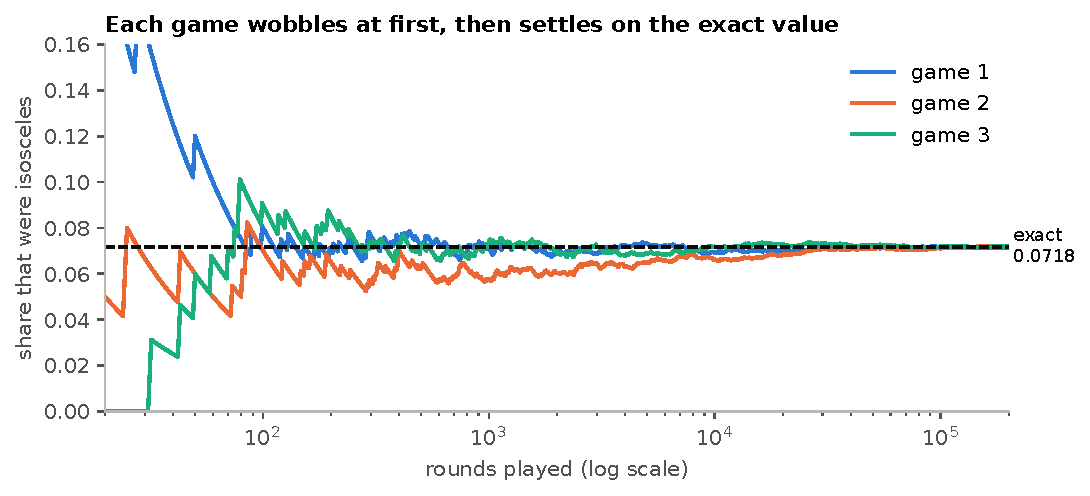
\includegraphics[width=0.95\linewidth]{fig16_running_rate}
  \caption{Three games, each of $200\,000$ rounds. After each round we plot the
  share of rounds won so far. Early on the share jumps around wildly; after
  tens of thousands of rounds every game hugs the dashed line, the exact value
  $0.0718$.}
\end{figure}

One game is still a little off. Playing many games shows how much one game varies,
and where the games are centred.

\begin{figure}[H]
  \centering
  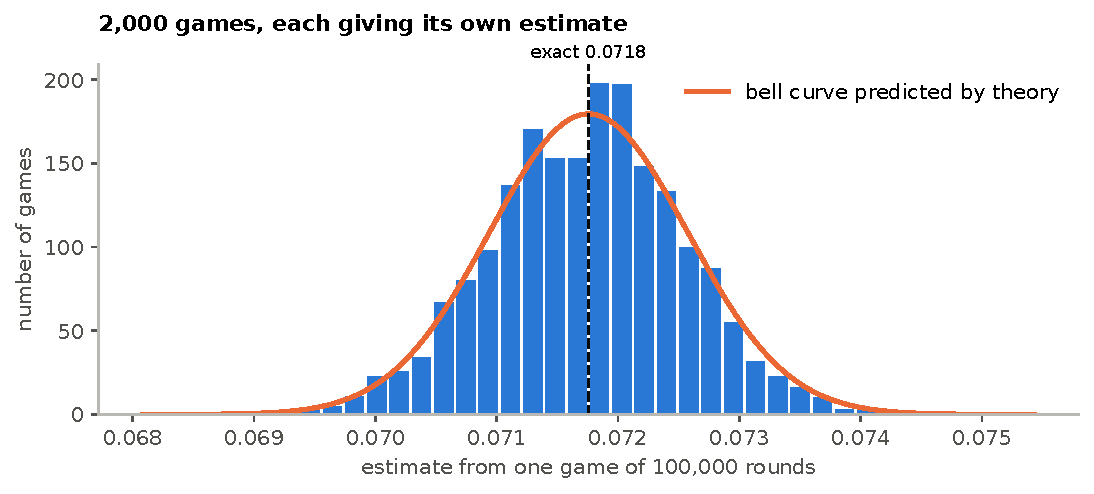
\includegraphics[width=0.95\linewidth]{fig17_histogram}
  \caption{$2000$ games of $100\,000$ rounds each. Each game gives its own
  estimate; the bars count how many games gave each value. They pile up around
  the exact value, in the bell shape that probability theory predicts
  (\orange{orange}).}
\end{figure}

The large experiment of the project ($10\,000$ games of $1\,000\,000$ rounds) gives
an average of $0.0717576$, against the exact $0.0717574$. A computer that checked
all $161\,700$ ways of picking three dots one by one also finds exactly $4448$
straight triples and $11\,284$ isosceles triangles.

% ---------------------------------------------------------------------------
\section{The whole story in eight lines}

\begin{enumerate}[nosep]
  \item The board has 100 dots; a round picks 3 of them.
  \item Squared lengths are whole numbers, so ``equal sides'' is an exact check.
  \item There are $161\,700$ ways to pick 3 dots; $4448$ are on a line and are
        redrawn, leaving $157\,252$ triangles.
  \item No triangle on the board is equilateral, so every isosceles triangle has
        one apex.
  \item The other two corners lie on a circle around the apex: every pair of dots on
        a circle is a triangle.
  \item Central dots have fuller circles than corner dots (257 pairs against 59).
  \item Pairs on a straight line through the apex are removed (1200 in all).
  \item That leaves $11\,284$ isosceles triangles, and a chance of
        $11\,284/157\,252\approx7.18\%$, confirmed by simulation.
\end{enumerate}

\end{document}
